\documentclass[hyperref={bookmarks=false},aspectratio=169]{beamer}
\usepackage{hyperref,ragged2e,amsmath,amssymb,url,bm}
\usepackage{graphicx,booktabs,array}
\usepackage{tikz}
\usetikzlibrary{shadows}
\usetikzlibrary{arrows.meta,positioning,calc,shapes.geometric,decorations.pathreplacing,matrix}
\graphicspath{{crops/}}
\usetheme{Goettingen}
% --- Paleta "Israel": celeste y azul del tejelet (Nm 15:38), oro del santuario, fondo crema ---
% (los nombres de color se conservan por compatibilidad con los cuerpos de las láminas: «ladrillo» = azul tejelet,
%  «cafe» = azul real, «cafeosc» = azul noche, «piedra» = celeste claro, «sepia» = azul pizarra)
\definecolor{cafe}{RGB}{26,82,150}
\definecolor{cafeosc}{RGB}{11,33,74}
\definecolor{tinta}{RGB}{20,32,56}
\definecolor{oro}{RGB}{206,162,52}
\definecolor{ladrillo}{RGB}{20,68,140}
\definecolor{piedra}{RGB}{234,243,251}
\definecolor{sepia}{RGB}{72,102,140}
\definecolor{celeste}{RGB}{96,166,222}
\setbeamercolor{structure}{fg=ladrillo}
\setbeamertemplate{sidebar canvas right}[vertical shading][top=celeste!75!ladrillo,middle=ladrillo,bottom=cafeosc]
\setbeamercolor{title in sidebar}{fg=oro!80!white}
\setbeamercolor{author in sidebar}{fg=piedra}
\setbeamercolor{section in sidebar}{fg=white}
\setbeamercolor{section in sidebar shaded}{fg=celeste!45!white}
\setbeamercolor{subsection in sidebar}{fg=white}
\setbeamercolor{subsection in sidebar shaded}{fg=celeste!45!white}
\let\raggedright\justifying
\definecolor{crema}{RGB}{250,245,230}
\setbeamertemplate{background canvas}[default]
\setbeamercolor{background canvas}{bg=crema}
\setbeamercolor{normal text}{fg=tinta}
\setbeamercolor{frametitle}{fg=ladrillo}
\setbeamerfont{frametitle}{series=\bfseries}
\setbeamertemplate{section in toc shaded}{\leavevmode{\color{sepia!85!black}\inserttocsection}\par}
\setbeamercolor{title}{fg=ladrillo}
\setbeamercolor{subtitle}{fg=cafe}
\setbeamercolor{item projected}{bg=cafe,fg=piedra}
\setbeamertemplate{itemize item}{\small\textcolor{oro!85!ladrillo}{$\blacktriangleright$}}
\setbeamertemplate{navigation symbols}{}
% --- Español + hebreo + griego (XeLaTeX) con fuentes empaquetadas en fonts/ ---
\usepackage[bidi=default]{babel}
\babelprovide[import,main]{spanish}
\babelprovide[import]{hebrew}
\babelprovide[import]{ancientgreek}
\babelfont[hebrew]{sf}[Path=fonts/, BoldFont=NotoHebrewSans-700.ttf]{NotoHebrewSans-400.ttf}
\babelfont[hebrew]{rm}[Path=fonts/, BoldFont=NotoHebrewSans-700.ttf]{NotoHebrewSans-400.ttf}
\babelfont[ancientgreek]{sf}[Path=fonts/]{GFSPorson.otf}
\babelfont[ancientgreek]{rm}[Path=fonts/]{GFSPorson.otf}
\newcommand{\heb}[1]{\mbox{\foreignlanguage{hebrew}{#1}}}
\newcommand{\grc}[1]{\foreignlanguage{ancientgreek}{#1}}
% --- Citas, imágenes, referencias ---
\usepackage[most]{tcolorbox}
\newtcolorbox{cita}[1][]{enhanced, colback=piedra!92!white, colframe=oro!90!ladrillo,
  boxrule=0pt, leftrule=2.5pt, arc=0pt, left=6pt, right=6pt, top=4pt, bottom=4pt,
  before skip=4pt, after skip=6pt, fontupper=\small\itshape, #1}
\newcommand{\fuente}[1]{\par\hfill{\upshape\bfseries\footnotesize\textcolor{ladrillo}{#1}}}
\newcommand{\imagen}[3][0.80]{%
  \centering\includegraphics[height=#1\textheight,width=\linewidth,keepaspectratio]{#2}\par\vspace{2pt}
  {\fontsize{5}{6}\selectfont\color{sepia}{\raggedleft\textit{Nota.} #3\par}}}
\makeatletter
\newcommand{\fotolado}[2]{%
  % Panel a la derecha, separado de la columna de texto (0.57): marco dorado, sombra y nota al pie.
  \begin{tikzpicture}[remember picture,overlay]
    \coordinate (fl) at ([xshift=\beamer@leftmargin+0.615\textwidth]current page.west);
    \coordinate (fr) at ([xshift=-\beamer@sidebarwidth-6pt]current page.east);
    \node[inner sep=0pt,anchor=center,draw=oro,line width=0.9pt,
      drop shadow={shadow xshift=1.2pt,shadow yshift=-1.2pt,opacity=0.30,fill=cafeosc}] (foto)
      at ([yshift=6pt]$(fl)!0.5!(fr)$)
      {\includegraphics[width=\dimexpr\paperwidth-\beamer@sidebarwidth-\beamer@leftmargin-0.615\textwidth-6pt\relax]{#1}};
    \node[anchor=north east,inner sep=0pt,text=sepia,font=\fontsize{4.6}{5.6}\selectfont,align=right,
      text width=\dimexpr\paperwidth-\beamer@sidebarwidth-\beamer@leftmargin-0.615\textwidth-6pt\relax]
      at ([yshift=-3pt]foto.south east) {\textit{Nota.} #2};
  \end{tikzpicture}}
\makeatother
\newcommand{\refapa}[1]{\par\hangindent=1.2em\hangafter=1\noindent #1\par\vspace{3pt}}
\usepackage{xurl}\urlstyle{same}
\newcommand{\destacar}[1]{\textbf{\textcolor{ladrillo}{#1}}}
% --- Piezas visuales de la serie: regla dorada bajo el título, notas y pies de figura ---
\addtobeamertemplate{frametitle}{}{\vspace{-3pt}{\color{oro}\rule{2.2cm}{1.1pt}}\vspace{1pt}}
\newtcolorbox{notalam}[1][Nota]{enhanced,colback=oro!10!white,colframe=oro!85!ladrillo,boxrule=0.5pt,arc=2pt,
  left=5pt,right=5pt,top=3pt,bottom=3pt,fonttitle=\bfseries\scriptsize,coltitle=cafeosc,colbacktitle=oro!30!white,
  fontupper=\scriptsize,title={#1},before skip=4pt,after skip=4pt}
\newtcolorbox{clave}[1][]{enhanced,colback=piedra,colframe=ladrillo,boxrule=0pt,leftrule=2.5pt,arc=0pt,
  left=5pt,right=5pt,top=3pt,bottom=3pt,fontupper=\scriptsize,before skip=4pt,after skip=4pt,#1}
\newcommand{\notafig}[1]{\par\vspace{2pt}{\fontsize{5}{6}\selectfont\color{sepia}\hfill\textit{Nota.} #1\par}}
\newcommand{\elabpropia}{\notafig{Elaboración propia.}}
\tikzset{hito/.style={circle,fill=oro,draw=white,line width=0.6pt,inner sep=1.6pt},
  etiq/.style={font=\tiny,text=tinta,align=center},
  flecha/.style={->,draw=oro!90!ladrillo,line width=1pt},
  bloque/.style={draw=ladrillo,line width=0.6pt,fill=piedra,rounded corners=3pt,font=\scriptsize,align=center,inner sep=4pt},
  bloqueoro/.style={draw=oro!90!ladrillo,line width=0.6pt,fill=oro!14!white,rounded corners=3pt,font=\scriptsize,align=center,inner sep=4pt},
  bloqueazul/.style={draw=cafeosc,fill=ladrillo,text=white,rounded corners=3pt,font=\scriptsize\bfseries,align=center,inner sep=4pt}}

\tikzset{caja/.style={draw=cafe!80!black,line width=0.7pt,top color=piedra!55!white,bottom color=piedra!92!oro,
  rounded corners=4pt,inner sep=5pt,font=\scriptsize,
  drop shadow={shadow xshift=0.7pt,shadow yshift=-0.8pt,opacity=0.25,fill=cafeosc}},
  >={Stealth[length=2.4mm,width=1.8mm]}, every picture/.style={line cap=round,line join=round}}
\newcommand{\precision}[1]{{\footnotesize\color{sepia}\textbf{Precisión:} #1}}
\newcommand{\pt}[2]{({#1-30},{#2-29})}
\title[Israel 3: Jueces--David]{\bfseries{Israel, el pueblo de Dios}}
\subtitle{Estudio 3. De los Jueces a David}
\author{}\institute{}\date{}
\titlegraphic{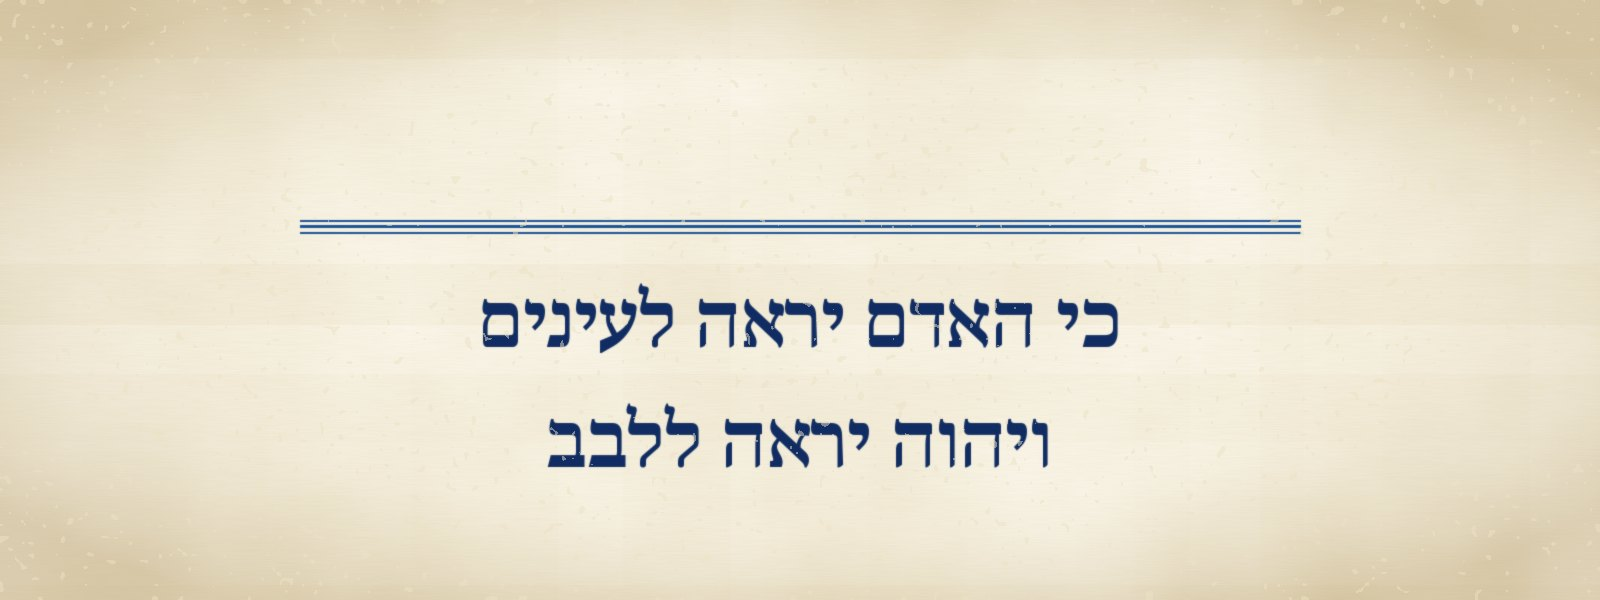
\includegraphics[width=0.85\linewidth,height=0.38\textheight,keepaspectratio]{portada.jpg}\\[-1pt]
  {\fontsize{5}{6}\selectfont\color{sepia}\textit{Nota.} Elaboración propia: 1~S 16:7 en texto hebreo consonántico (BHS).}}
\begin{document}
\frame{\titlepage}

% ===================================================
\section{Introducción}
\begin{frame}{¿Cansados de ser distintos?}
\begin{columns}[t,onlytextwidth]
\begin{column}{0.50\textwidth}
\begin{cita}Vosotros me seréis un reino de sacerdotes y una nación santa.\fuente{(Éx 19:6)}\end{cita}
\begin{cita}Constitúyenos ahora un rey que nos juzgue, como tienen todas las naciones.\fuente{(1~S 8:5)}\end{cita}
\begin{cita}No ha desechado Dios a su pueblo.\fuente{(Ro 11:2; cf. 1~S 12:22)}\end{cita}
\end{column}
\begin{column}{0.47\textwidth}\small
\destacar{Una ruina interna.} La vocación se quiebra \emph{desde dentro}: levitas, sacerdotes y tribus hacen «lo recto ante sus ojos» (Dt 12:8; Jue 21:25).\par\medskip
\destacar{Una promesa en pie.} Libertadores, un remanente, una moabita en el linaje de Judá y el anuncio de un rey \emph{ungido} (1~S 2:10).\par\medskip
{\scriptsize\color{sepia}Las citas bíblicas son traducción propia desde el texto hebreo (BHS) y griego (NA28). Numeración española [hebrea] cuando difiere.}
\end{column}
\end{columns}
\end{frame}

\begin{frame}{Los ejes de la serie en esta etapa}
\centering
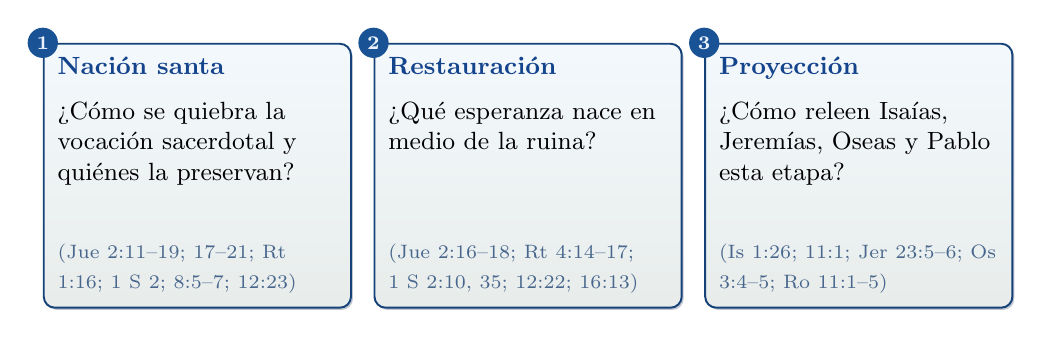
\begin{tikzpicture}
 \foreach \x/\n/\t/\d/\r in {0/1/{Nación santa}/{¿Cómo se quiebra la vocación sacerdotal y quiénes la preservan?}/{Jue 2:11--19; 17--21; Rt 1:16; 1~S 2; 8:5--7; 12:23},
   4.2/2/{Restauración}/{¿Qué esperanza nace en medio de la ruina?}/{Jue 2:16--18; Rt 4:14--17; 1~S 2:10, 35; 12:22; 16:13},
   8.4/3/{Proyección}/{¿Cómo releen Isaías, Jeremías, Oseas y Pablo esta etapa?}/{Is 1:26; 11:1; Jer 23:5--6; Os 3:4--5; Ro 11:1--5}}{
  \node[caja,anchor=north] (b\n) at (\x,0) {\parbox[t][3.0cm][t]{3.55cm}{\RaggedRight
    {\small\textbf{\textcolor{ladrillo}{\t}}}\\[5pt]\small \d\par\vfill{\scriptsize\color{sepia}(\r)}}};
  \node[circle,fill=cafe,text=piedra,font=\scriptsize\bfseries,inner sep=1.6pt] at (b\n.north west) {\n};}
\end{tikzpicture}\par\vspace{6pt}
{\scriptsize\color{sepia}En esta etapa «Israel» designa a todo el pueblo; la distinción Israel\,/\,Judá asoma al final (1~S 11:8; 18:16; 2~S 2:4, 9--10).}
\end{frame}

% ===================================================
\section{Cronología}
\begin{frame}{Secuencia de la etapa}
\centering
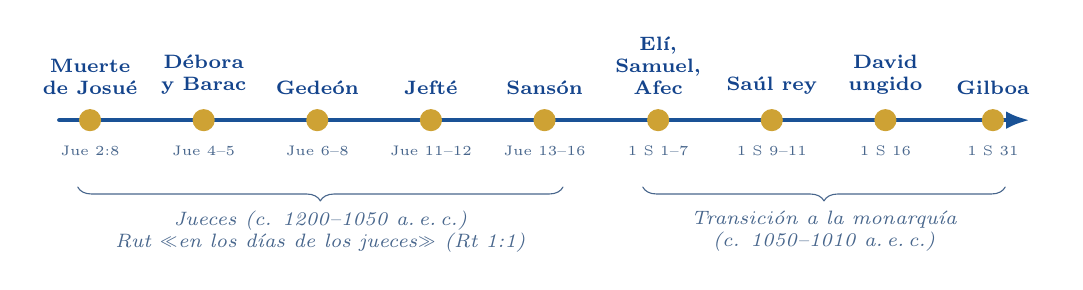
\begin{tikzpicture}[x=0.78cm]
\draw[line width=1.6pt,cafe,-{Latex[length=3mm]}] (0,0) -- (15.8,0);
\foreach \x/\t/\b in {0.5/{Muerte de Josué}/{Jue 2:8},
                      2.35/{Débora y Barac}/{Jue 4--5},
                      4.2/{Gedeón}/{Jue 6--8},
                      6.05/{Jefté}/{Jue 11--12},
                      7.9/{Sansón}/{Jue 13--16},
                      9.75/{Elí, Samuel, Afec}/{1~S 1--7},
                      11.6/{Saúl rey}/{1~S 9--11},
                      13.45/{David ungido}/{1~S 16},
                      15.2/{Gilboa}/{1~S 31}}{
  \fill[oro] (\x,0) circle (4pt);
  \node[above,font=\scriptsize\bfseries,text=ladrillo,text width=1.35cm,align=center] at (\x,0.2) {\t};
  \node[below,font=\tiny,text=sepia,text width=1.35cm,align=center] at (\x,-0.2) {\b};}
\draw[decorate,decoration={brace,amplitude=5pt,mirror},sepia] (0.3,-0.85) -- (8.2,-0.85) node[midway,below=5pt,font=\scriptsize\itshape,align=center]{Jueces (c. 1200--1050 a.\,e.\,c.)\\Rut «en los días de los jueces» (Rt 1:1)};
\draw[decorate,decoration={brace,amplitude=5pt,mirror},sepia] (9.5,-0.85) -- (15.4,-0.85) node[midway,below=5pt,font=\scriptsize\itshape,align=center]{Transición a la monarquía\\(c. 1050--1010 a.\,e.\,c.)};
\end{tikzpicture}\par\vspace{4pt}
{\fontsize{5}{6}\selectfont\color{sepia}\raggedleft\textit{Nota.} Elaboración propia. Secuencia narrativa; las fechas absolutas son aproximadas y están en debate.\par}
\end{frame}

\begin{frame}{Fechas en debate}
\begin{columns}[t,onlytextwidth]
\begin{column}{0.48\textwidth}\small
\textbf{\textcolor{cafe}{¿Cuánto duró el período?}}
\begin{itemize}
\item \textbf{1~R 6:1}: 480 años del Éxodo al 4.º año de Salomón.
\item \textbf{Suma de Jueces}: c. 390 años en sucesión (cálculo propio); sumando Elí, Saúl y David, la cifra se excede.
\item Explicación habitual: \destacar{jueces regionales superpuestos} (Jue 10:7: Amón al este, filisteos al oeste).
\item Seder Olam encaja las cifras en los 480 años.
\end{itemize}
\end{column}
\begin{column}{0.50\textwidth}
\textbf{\small\textcolor{cafe}{Dos problemas textuales}}\par\smallskip
\scriptsize\renewcommand{\arraystretch}{1.2}
\begin{tabular}{>{\RaggedRight\arraybackslash}p{1.6cm}>{\RaggedRight\arraybackslash}p{4.1cm}}
\toprule
\textbf{Texto} & \textbf{Problema}\\\midrule
Hch 13:20 & NA28: 450 años \emph{antes} de los jueces (Egipto, desierto, conquista). Texto bizantino (RV): 450 años \emph{de} jueces.\\
1~S 13:1 & TM: Saúl «tenía un año» y «reinó dos años»: cifras perdidas. Hch 13:21: 40 años.\\
\bottomrule
\end{tabular}\par\smallskip
\precision{Saúl c. 1025--1010; David desde c. 1010 a.\,e.\,c. (convencional).}
\end{column}
\end{columns}
\end{frame}

% ===================================================
\section{Arqueología}
\begin{frame}{El escenario de la etapa}
\begin{columns}[c,onlytextwidth]
\begin{column}{0.47\textwidth}\centering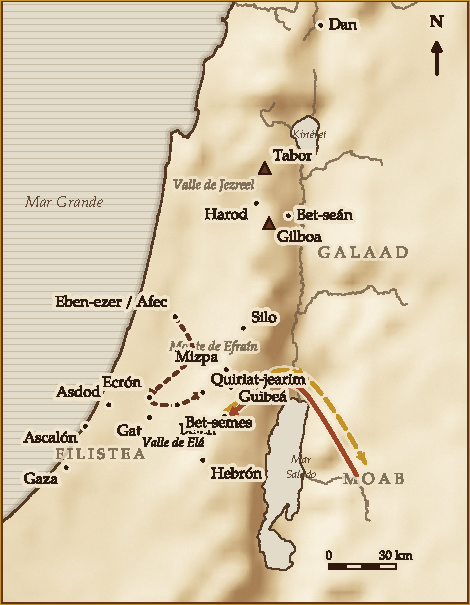
\includegraphics[width=\linewidth,height=0.86\textheight,keepaspectratio]{mapa_jueces.pdf}\par\vspace{1pt}{\fontsize{4.5}{5.5}\selectfont\color{sepia}\textit{Nota.} Elaboración propia (GSHHS/WDB, Basemap); ubicaciones aproximadas.\par}\end{column}
\begin{column}{0.51\textwidth}\scriptsize\RaggedRight
{\scriptsize\RaggedRight
\tikz[baseline=-0.6ex]\draw[oro,line width=1.5pt,line cap=round,dash pattern=on 3.4pt off 1.8pt](0,0)--(0.6,0);~Elimelec y Noemí a Moab (Rt 1:1)\par
\tikz[baseline=-0.6ex]\draw[ladrillo,line width=1.5pt,line cap=round](0,0)--(0.6,0);~Noemí y Rut regresan a Belén (Rt 1:22)\par
\tikz[baseline=-0.6ex]\draw[cafe,line width=1.5pt,line cap=round,dash pattern=on 1.2pt off 1.4pt](0,0)--(0.6,0);~El arca: Eben-ezer $\to$ Asdod… $\to$ Quiriat-jearim (1 S 4–7)\par}
\medskip

\textbf{\textcolor{cafe}{Sierra central}}: Silo, Mizpa, Guibeá; las aldeas israelitas del Hierro~I.\par\smallskip
\textbf{\textcolor{cafe}{Pentápolis filistea}}: Gaza, Asdod, Ascalón, Gat, Ecrón (Jue 3:3).\par\smallskip
\textbf{\textcolor{cafe}{Frontera}}: Bet-semes y el valle de Elá (Qeiyafa).\par\smallskip
\textbf{\textcolor{cafe}{Norte}}: Tabor (Jue 4), Harod (Jue 7), Gilboa y Bet-seán (1~S 31).\par\smallskip
\textbf{\textcolor{cafe}{Rut}}: de Belén a Moab y de regreso, cruzando el Jordán junto a Jericó.\par\medskip
\precision{Eben-ezer y otros sitios tienen identificación debatida.}
\end{column}
\end{columns}
\end{frame}

\begin{frame}{Aldeas y filisteos}
\centering
\begin{tikzpicture}
 \foreach \x/\n/\t/\d/\r in {0/1/{Aldeas de la sierra}/{Más de 250 aldeas sin muralla en el Hierro~I; casa de cuatro espacios (\emph{bet av}).}/{Finkelstein, 1988; Stager, 1985},
   3.15/2/{Medinet Habu}/{Ramsés~III combate a los Pueblos del Mar, entre ellos los \emph{Peleset} (\heb{פְּלִשְׁתִּים}).}/{c. 1177 a.\,e.\,c.; Dothan, 1982},
   6.3/3/{Ecrón}/{«Akish, hijo de Padi, rey de Ecrón»: el nombre de Aquis de Gat (1~S 27:2). Siglo \textsc{vii}.}/{Gitin et~al., 1997},
   9.45/4/{Gat}/{Ostracón con \emph{’LWT} y \emph{WLT}, nombres cercanos a «Goliat». No es Goliat.}/{Maeir et~al., 2008}}{
  \node[caja,anchor=north] (b\n) at (\x,0) {\parbox[t][3.2cm][t]{2.65cm}{\RaggedRight
    {\small\textbf{\textcolor{ladrillo}{\t}}}\\[4pt]\scriptsize \d\par\vfill{\tiny\color{sepia}(\r)}}};
  \node[circle,fill=cafe,text=piedra,font=\scriptsize\bfseries,inner sep=1.6pt] at (b\n.north west) {\n};}
\end{tikzpicture}\par\vspace{5pt}
\begin{minipage}{0.95\linewidth}\scriptsize \textbf{Debate:} la ausencia de huesos de cerdo en la sierra se ha leído como marcador israelita (Faust, 2006); Hesse y Wapnish (1997) advierten que depende también del clima y la economía.\end{minipage}
\end{frame}

\begin{frame}{Silo, Bet-semes y Qeiyafa}
\begin{columns}[t,onlytextwidth]
\begin{column}{0.49\textwidth}\small
\begin{itemize}
\item \textbf{Silo}: incendio a mediados del s. \textsc{xi} a.\,e.\,c. (Finkelstein et~al., 1993). ¿Tras Afec? Samuel calla; Jer 7:12 y Sal 78:60 lo recuerdan.
\item \textbf{Bet-semes}: frontera con Ecrón, adonde vuelve el arca (1~S 6).
\item \textbf{\emph{Pim}} (1~S 13:21): palabra oscura aclarada por pesas inscritas \emph{pym}.
\end{itemize}
\end{column}
\begin{column}{0.49\textwidth}\small
\textbf{\textcolor{cafe}{Khirbet Qeiyafa}}: fortaleza sobre el valle de Ela, c.~1020--980 a.\,e.\,c.
\begin{itemize}
\item Garfinkel: ciudad de Judá del tiempo de David (¿Saaraim, 1~S 17:52?).
\item Finkelstein y Fantalkin (2012): entidad del norte, quizá la de Saúl.
\item Otros: cananea o filistea.
\end{itemize}
\precision{la «cronología baja» de Finkelstein reduce el reino de David; Mazar (1990) y otros la rechazan.}
\end{column}
\end{columns}
\end{frame}

% ===================================================
\section{Jueces y Rut}
\begin{frame}{El ciclo: una espiral}
\begin{columns}[c,onlytextwidth]
\begin{column}{0.52\textwidth}
\centering
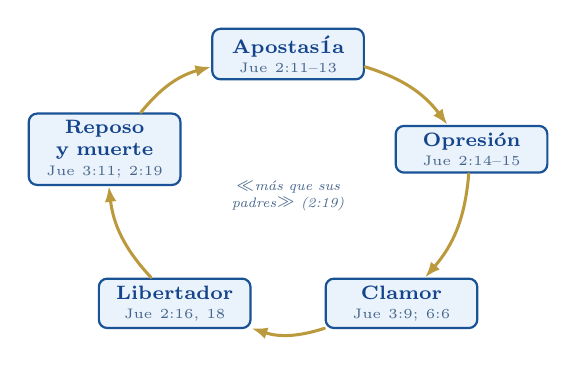
\begin{tikzpicture}[every node/.style={font=\scriptsize}]
\foreach \a/\t/\r [count=\i] in {90/{Apostasía}/{2:11--13},18/{Opresión}/{2:14--15},-54/{Clamor}/{3:9; 6:6},-126/{Libertador}/{2:16, 18},162/{Reposo y muerte}/{3:11; 2:19}}{
  \node[draw=cafe,line width=0.8pt,fill=piedra,rounded corners=3pt,text width=1.75cm,align=center,inner sep=2.5pt] (c\i) at ({2.45*cos(\a)},{1.75*sin(\a)}) {\textbf{\textcolor{ladrillo}{\t}}\\[-1pt]{\tiny\color{sepia}Jue \r}};}
\foreach \a/\b in {1/2,2/3,3/4,4/5,5/1}{\draw[-{Latex[length=2mm]},oro!90!ladrillo,line width=1.1pt] (c\a) to[bend left=18] (c\b);}
\node[text width=1.9cm,align=center,font=\tiny\itshape,text=sepia] at (0,-0.05) {«más que sus padres» (2:19)};
\end{tikzpicture}
\end{column}
\begin{column}{0.45\textwidth}
\begin{cita}[fontupper=\scriptsize\itshape]YHWH levantó jueces que los libraron [\ldots]. Pero cuando moría el juez, volvían a corromperse más que sus padres.\fuente{(Jue 2:16, 19)}\end{cita}
\scriptsize
\begin{itemize}
\item «Reposó la tierra» desaparece tras Gedeón (3:11; 5:31; 8:28).
\item Las tribus terminan en guerra civil (12:1--6; Jue 20).
\item \heb{שֹׁפֵט} (\emph{shofet}): libertador y gobernante; el Juez es YHWH (11:27).
\end{itemize}
\end{column}
\end{columns}
\end{frame}

\begin{frame}{Los jueces mayores}
\centering\scriptsize\renewcommand{\arraystretch}{1.2}
\begin{tabular}{>{\RaggedRight\arraybackslash}p{1.8cm}>{\RaggedRight\arraybackslash}p{1.8cm}>{\RaggedRight\arraybackslash}p{2.1cm}>{\RaggedRight\arraybackslash}p{1.4cm}>{\RaggedRight\arraybackslash}p{3.9cm}}
\toprule
\textbf{Juez} & \textbf{Tribu} & \textbf{Opresor} & \textbf{Texto} & \textbf{Rasgo}\\\midrule
Otoniel & Judá & Cusán-risataim & 3:7--11 & Modelo inicial; reposo de 40 años\\
Aod & Benjamín & Eglón de Moab & 3:12--30 & Libertador zurdo; reposo de 80 años\\
Débora y Barac & Efraín\,/ Neftalí & Jabín y Sísara & 4--5 & Profetisa y jueza; Jael completa la victoria\\
Gedeón & Manasés & Madián & 6--8 & Rechaza la corona; su efod es tropiezo\\
Jefté & Galaad & Amón & 10:6--12:7 & Voto temerario; guerra contra Efraín\\
Sansón & Dan & Filisteos & 13--16 & Nazareo; vive «según sus ojos»\\
\bottomrule
\end{tabular}\par\vspace{8pt}
{\small\itshape\color{sepia}De Otoniel a Sansón decaen la talla de los jueces y la unidad de las tribus.}
\end{frame}

\begin{frame}{Débora y Gedeón}
\begin{columns}[t,onlytextwidth]
\begin{column}{0.48\textwidth}
\textbf{\textcolor{cafe}{El cántico de Débora (Jue 5)}}\par\smallskip
\small Para muchos, junto con Éx 15, uno de los poemas más antiguos de la Biblia (Cross y Freedman, 1997); otros lo datan más tarde.
\scriptsize
\begin{itemize}
\item Alaba: Efraín, Benjamín, Maquir, Zabulón, Isacar, Neftalí.
\item Reprocha: Rubén, Galaad, Dan, Aser. Maldice a Meroz (5:23).
\item No menciona a Judá ni a Simeón.
\end{itemize}
\begin{cita}[fontupper=\scriptsize\itshape]Los que le aman sean como el sol cuando sale en su fuerza.\fuente{(Jue 5:31)}\end{cita}
\end{column}
\begin{column}{0.49\textwidth}
\centering{\heb{יְהוָה יִמְשֹׁל בָּכֶם}}\par\smallskip
\begin{cita}No reinaré yo sobre vosotros, ni mi hijo reinará sobre vosotros; YHWH reinará sobre vosotros.\fuente{(Jue 8:23)}\end{cita}
\scriptsize
\begin{itemize}
\item Pero su efod se vuelve «tropiezo» (8:27).
\item Abimelec, «mi padre es rey», se hace rey (Jue 9); fábula de Jotam.
\item «Como el día de Madián» será figura profética (Is 9:4 [9:3]).
\end{itemize}
\end{column}
\end{columns}
\end{frame}

\begin{frame}{Jefté y Sansón}
\begin{columns}[t,onlytextwidth]
\begin{column}{0.48\textwidth}\small
\textbf{\textcolor{cafe}{Jefté (Jue 11--12)}}
\begin{itemize}
\item Conoce la historia del Éxodo (11:12--28), pero su voto sigue la lógica de los dioses vecinos.
\item Josefo: la sacrificó, y condena el acto. Kimji: consagrada a la virginidad (11:39).
\item \heb{שִׁבֹּלֶת}\,/\,\heb{סִבֹּלֶת}: Israel ya mata a Israel (12:6).
\end{itemize}
\end{column}
\begin{column}{0.49\textwidth}\small
\textbf{\textcolor{cafe}{Sansón (Jue 13--16)}}
\begin{itemize}
\item \heb{נְזִיר אֱלֹהִים} (\emph{nezir Elohim}) desde el vientre (13:5).
\item Quebranta uno a uno los signos de su consagración: cadáver, banquete, cabello.
\item «Tómamela, porque es recta a mis ojos» (\heb{יָשְׁרָה בְעֵינָי}, 14:3).
\item Aun así, figura en Heb 11:32.
\end{itemize}
\end{column}
\end{columns}\par\medskip
{\small\itshape\color{sepia}\centering En Sansón se reconoce al Israel de la época: consagrado desde su origen, vive como las naciones sin perder su llamado.\par}
\end{frame}

\begin{frame}{Un levita a sueldo (Jue 17--18)}
\begin{columns}[t,onlytextwidth]
\begin{column}{0.50\textwidth}
\begin{cita}Ahora sé que YHWH me prosperará, porque tengo un levita por sacerdote.\fuente{(Jue 17:13)}\end{cita}
\small
\begin{itemize}
\item Micaía: ídolo, efod, terafines y un levita de Belén por diez siclos al año.
\item Dan roba el ídolo y al levita, arrasa Lais y funda un santuario «hasta el cautiverio de la tierra» (18:30).
\end{itemize}
\end{column}
\begin{column}{0.47\textwidth}
\begin{tcolorbox}[colback=piedra,colframe=cafe,boxrule=0.8pt,arc=3pt,fontupper=\scriptsize,title={\scriptsize\bfseries Precisión textual (18:30)},colbacktitle=oro!35,coltitle=cafe]
«Jonatán, hijo de Gersón, hijo de \emph{Manasés}»: la \emph{nun} de \heb{מנשה} va suspendida; sin ella se lee \heb{משה}, «Moisés». El Talmud: se añadió para no avergonzar a Moisés (Bava Batra 109b).
\end{tcolorbox}
\scriptsize En ese mismo Dan pondrá Jeroboam su becerro (1~R 12:29), antesala del destierro asirio (Estudio~5).
\end{column}
\end{columns}
\end{frame}

\begin{frame}{No había rey en Israel}
\fotolado{panel_jue21.jpg}{Elaboración propia: Jue 21:25 en texto hebreo consonántico (BHS).}
\begin{columns}[c,onlytextwidth]
\begin{column}{0.57\textwidth}
\begin{cita}En aquellos días no había rey en Israel; cada uno hacía lo que era recto ante sus propios ojos.\fuente{(Jue 21:25; cf. 17:6)}\end{cita}
\scriptsize
\begin{itemize}
\item \textbf{Guibeá} reproduce la escena de Sodoma (Jue 19:22; Gn 19:4--5): Israel se ha vuelto Canaán.
\item \textbf{Benjamín} casi desaparece: «que falte hoy de Israel una tribu» (21:3).
\item \textbf{Dt 12:8}: \heb{אִישׁ כָּל־הַיָּשָׁר בְּעֵינָיו} frente a lo recto ante los ojos de YHWH (12:25).
\item \textbf{Os 10:9}: «desde los días de Guibeá has pecado, oh Israel».
\end{itemize}
\end{column}
\begin{column}{0.41\textwidth}\end{column}
\end{columns}
\end{frame}

\begin{frame}{Tu pueblo será mi pueblo}
\fotolado{panel_rt1.jpg}{Elaboración propia: Rt 1:16 en texto hebreo consonántico (BHS).}
\begin{columns}[c,onlytextwidth]
\begin{column}{0.57\textwidth}
\begin{cita}Adonde tú vayas, iré yo; y donde tú pases la noche, la pasaré yo. Tu pueblo será mi pueblo, y tu Dios, mi Dios.\fuente{(Rt 1:16)}\end{cita}
\scriptsize
\begin{itemize}
\item «En los días en que juzgaban los jueces» (1:1), en la Belén de Jue 17--21; aquí, en cambio, una moabita vive como israelita fiel.
\item Un orden significativo: \destacar{primero el pueblo, después Dios}.
\item \heb{חֶסֶד} (\emph{jésed}): lealtad más allá de lo debido (1:8; 2:20; 3:10).
\item \heb{כָּנָף}: «bajo sus alas» (2:12) y «extiende tu manto» (3:9).
\end{itemize}
\end{column}
\begin{column}{0.41\textwidth}\end{column}
\end{columns}
\end{frame}

\begin{frame}{El redentor y la moabita}
\begin{columns}[t,onlytextwidth]
\begin{column}{0.49\textwidth}\small
\textbf{\textcolor{cafe}{Booz, el \emph{go'el}}} (\heb{גֹּאֵל})
\begin{itemize}
\item Rescata la tierra y el nombre del pariente (Lv 25:25; cf. Dt 25:5--10).
\item «No te ha dejado hoy sin redentor» (Rt 4:14).
\item \heb{הוּא אֲבִי־יִשַׁי אֲבִי דָוִד}: «padre de Isaí, padre de David» (4:17).
\item Rut en la genealogía del Mesías (Mt 1:5).
\end{itemize}
\end{column}
\begin{column}{0.49\textwidth}
\textbf{\small\textcolor{cafe}{¿Y Dt 23:3 [23:4]?}}\par\smallskip
\begin{cita}[fontupper=\scriptsize\itshape]No entrará amonita ni moabita en la congregación de YHWH.\fuente{(Dt 23:3 [23:4])}\end{cita}
\scriptsize
Mishná (Yevamot 8:3) y Talmud (Yevamot 76b--77a): «\emph{moabita, y no moabitesa}». Es interpretación rabínica, no distinción explícita de la Torá; Esd 9--10 y Neh 13:1--3 aplican la ley con más rigor.
\end{column}
\end{columns}
\end{frame}

% ===================================================
\section{Samuel}
\begin{frame}{El cántico de Ana}
\fotolado{panel_1s2.jpg}{Elaboración propia: 1~S 2:10 en texto hebreo consonántico (BHS).}
\begin{columns}[c,onlytextwidth]
\begin{column}{0.57\textwidth}
\begin{cita}YHWH juzgará los confines de la tierra; dará poder a su rey y exaltará el poder de su ungido.\fuente{(1~S 2:10)}\end{cita}
\scriptsize
\begin{itemize}
\item Una estéril, como Sara: Dios la «visita» (\heb{פָּקַד}, 1~S 2:21; Gn 21:1).
\item Poema de la inversión: «levanta del polvo al pobre» (2:8).
\item Habla de «su rey» cuando Israel aún no tiene ninguno.
\item \heb{מְשִׁיחוֹ} (\emph{meshijó}): primera vez que el «ungido» es un rey.
\end{itemize}
\end{column}
\begin{column}{0.41\textwidth}\end{column}
\end{columns}
\end{frame}

\begin{frame}{«Su ungido»: del hebreo a Lucas}
\centering
\begin{tikzpicture}[node distance=0.9cm]
\node[caja,text width=3.3cm,align=center] (h) {\textbf{Hebreo (1~S 2:10)}\\[3pt]\heb{וְיָרֵם קֶרֶן מְשִׁיחוֹ}\\[2pt]«exaltará el cuerno\\de su ungido»};
\node[caja,text width=3.3cm,align=center,right=of h] (g) {\textbf{LXX}\\[3pt]\grc{ὑψώσει κέρας χριστοῦ αὐτοῦ}\\[2pt]\emph{mashíaj} $\to$ \grc{χριστός}};
\node[caja,text width=3.3cm,align=center,right=of g] (p) {\textbf{Lucas (1:69)}\\[3pt]\grc{ἤγειρεν κέρας σωτηρίας}\\[2pt]«en la casa de David»};
\draw[-{Latex[length=2.5mm]},oro!90!ladrillo,line width=1.4pt] (h) -- (g);
\draw[-{Latex[length=2.5mm]},oro!90!ladrillo,line width=1.4pt] (g) -- (p);
\end{tikzpicture}\par\vspace{8pt}
{\small\itshape\color{sepia}María canta como Ana: «quitó de los tronos a los poderosos y exaltó a los humildes» (Lc 1:52; cf. 1~S 2:7--8).}\par\vspace{6pt}
\begin{minipage}{0.92\linewidth}\precision{4QSam\textsuperscript{a} añade en 1~S 1:22 que Samuel será «nazareo para siempre»; la LXX de 1~S 2:10 inserta un texto cercano a Jer 9:23--24 [9:22--23]. Se traduce el TM.}\end{minipage}
\end{frame}

\begin{frame}{Icabod y Eben-ezer}
\begin{columns}[t,onlytextwidth]
\begin{column}{0.49\textwidth}
\centering{\heb{אִי־כָבוֹד \foreignlanguage{spanish}{[\ldots]} גָּלָה כָבוֹד מִיִּשְׂרָאֵל}}\par\smallskip
\begin{cita}Y llamó al niño Icabod, diciendo: ¡Se ha ido la gloria de Israel!\fuente{(1~S 4:21)}\end{cita}
\scriptsize
\begin{itemize}
\item Hijos de Elí: «no conocían a YHWH» (2:12).
\item Afec: el arca usada como amuleto (4:3).
\item \heb{גָּלָה}: la gloria «va al exilio».
\item Dagón cae; el arca vuelve sola a Bet-semes (5--6).
\end{itemize}
\end{column}
\begin{column}{0.49\textwidth}
\centering{\heb{עַד־הֵנָּה עֲזָרָנוּ יְהוָה}}\par\smallskip
\begin{cita}Y le puso por nombre Eben-ezer, diciendo: Hasta aquí nos ayudó YHWH.\fuente{(1~S 7:12)}\end{cita}
\scriptsize Mizpa: «quitad los dioses ajenos» (7:3); ayuno, confesión, intercesión. Con el arca como objeto, Israel perdió; al volver a Dios, fue librado.\par\smallskip
\precision{1~S 2:35 promete «un sacerdote fiel» que andará «delante de mi ungido».}
\end{column}
\end{columns}
\end{frame}

\begin{frame}{«Como todas las naciones»}
\centering
\begin{tikzpicture}
 \foreach \x/\n/\t/\d/\r in {0/1/{Éx 19:6}/{«Reino de sacerdotes y nación santa»: un pueblo distinto para las naciones.}/{Nm 23:9},
   4.2/2/{Dt 17:14--20}/{Un rey \emph{que Dios escoja}, sin caballos, mujeres ni oro, que lea la Torá cada día.}/{Gn 17:6; 49:10},
   8.4/3/{1~S 8:5, 20}/{\heb{כְּכָל־הַגּוֹיִם}: «un rey [\ldots] como todas las naciones».}/{8:7: «a mí me han desechado»}}{
  \node[caja,anchor=north] (b\n) at (\x,0) {\parbox[t][2.75cm][t]{3.55cm}{\RaggedRight
    {\small\textbf{\textcolor{ladrillo}{\t}}}\\[5pt]\small \d\par\vfill{\scriptsize\color{sepia}(\r)}}};
  \node[circle,fill=cafe,text=piedra,font=\scriptsize\bfseries,inner sep=1.6pt] at (b\n.north west) {\n};}
\end{tikzpicture}\par\vspace{8pt}
\begin{minipage}{0.95\linewidth}\small La Torá prevé la monarquía; lo que está en juego es el \destacar{modelo}: un rey a la manera de las naciones, en lugar de un rey sujeto a la Torá en un pueblo llamado a ser distinto.\end{minipage}
\end{frame}

% ===================================================
\section{Saúl y David}
\begin{frame}{Saúl: obedecer es mejor}
\begin{columns}[t,onlytextwidth]
\begin{column}{0.49\textwidth}\small
\begin{itemize}
\item Benjaminita, ungido \heb{נָגִיד} (\emph{naguid}) sobre la heredad de YHWH (10:1).
\item Libra a Jabes, la ciudad arrasada en Jue 21 (1~S 11).
\item Gilgal: ofrece él mismo el holocausto (13:8--12). «YHWH se ha buscado un hombre conforme a su corazón» (13:14).
\item Amalec: perdona a Agag (1~S 15). El reino es «rasgado» (15:28).
\end{itemize}
\end{column}
\begin{column}{0.49\textwidth}
\centering{\heb{הִנֵּה שְׁמֹעַ מִזֶּבַח טוֹב}}\par\smallskip
\begin{cita}Ciertamente obedecer es mejor que el sacrificio, y prestar atención, mejor que la grasa de los carneros.\fuente{(1~S 15:22)}\end{cita}
\begin{cita}[fontupper=\scriptsize\itshape]YHWH no desamparará a su pueblo, por causa de su gran nombre.\fuente{(1~S 12:22)}\end{cita}
\scriptsize LXX: \grc{οὐκ ἀπώσεται κύριος τὸν λαὸν αὐτοῦ} $\to$ Ro 11:1--2.
\end{column}
\end{columns}
\end{frame}

\begin{frame}{David: el menor de Belén}
\begin{columns}[t,onlytextwidth]
\begin{column}{0.49\textwidth}
\centering{\heb{וַיהוָה יִרְאֶה לַלֵּבָב}}\par\smallskip
\begin{cita}El hombre mira lo que está delante de sus ojos, pero YHWH mira el corazón.\fuente{(1~S 16:7)}\end{cita}
\scriptsize
\begin{itemize}
\item Contrapunto al estribillo de Jueces: Dios elige mirando el corazón.
\item El menor, con las ovejas; el Espíritu viene sobre él «desde aquel día» (16:13).
\item El ungido de 2:10 recibe un nombre.
\end{itemize}
\end{column}
\begin{column}{0.49\textwidth}
\centering{\heb{כִּי יֵשׁ אֱלֹהִים לְיִשְׂרָאֵל}}\par\smallskip
\begin{cita}Toda la tierra sabrá que hay Dios en Israel [\ldots], porque de YHWH es la batalla.\fuente{(1~S 17:46--47)}\end{cita}
\scriptsize Una victoria con fin misionero: Éx 19:6 en boca de un pastor.\par\smallskip
\precision{Goliat mide «seis codos y un palmo» en el TM; «cuatro codos y un palmo» en LXX, 4QSam\textsuperscript{a} y Josefo. Cf. 2~S 21:19 y 1~Cr 20:5.}
\end{column}
\end{columns}
\end{frame}

\begin{frame}{Jonatán, Gilboa y dos casas}
\begin{columns}[t,onlytextwidth]
\begin{column}{0.50\textwidth}\small
\begin{itemize}
\item \textbf{Jonatán}: «tú reinarás sobre Israel, y yo seré segundo» (23:17).
\item \textbf{Nob}: Saúl mata a los sacerdotes (22:18; cf. 2:31--33).
\item \textbf{David perdona} al «ungido de YHWH» (\heb{מְשִׁיחַ יְהוָה}, 24:6 [24:7]).
\item \textbf{Abigail}: Dios le hará «casa firme» (\heb{בַּיִת נֶאֱמָן}, 25:28).
\item \textbf{Endor y Gilboa} (1~S 28; 31): «¡Cómo han caído los valientes!» (2~S 1:19).
\end{itemize}
\end{column}
\begin{column}{0.47\textwidth}
\begin{tcolorbox}[colback=piedra,colframe=ladrillo,boxrule=0.8pt,arc=3pt,fontupper=\small]
\textbf{\textcolor{cafe}{Judá e Israel}}\par\smallskip
David, rey de «la casa de Judá» en Hebrón (2~S 2:4); Is-boset, rey de «todo Israel» (2:9--10).\par\smallskip
\scriptsize Por primera vez, dos entidades políticas (ya insinuadas en 1~S 11:8 y 18:16). La división definitiva, en el Estudio~4.
\end{tcolorbox}
\end{column}
\end{columns}
\end{frame}

% ===================================================
\section{Vocación}
\begin{frame}{La vocación quebrada y preservada}
\begin{columns}[t,onlytextwidth]
\begin{column}{0.49\textwidth}
\textbf{\textcolor{ladrillo}{Quebrada}}
\scriptsize
\begin{itemize}
\item \textbf{Cananeización}: los baales (Jue 2:11--13); su raíz está en Balac y Balaam (Nm 22--25; Ap 2:14).
\item \textbf{Sacerdocio vendido}: el levita de Micaía; los hijos de Elí.
\item \textbf{Culto como magia}: el arca amuleto; Saúl en Gilgal; Endor.
\item \textbf{Israel como Sodoma}: Guibeá.
\item \textbf{Como las naciones}: 1~S 8 frente a Nm 23:9.
\end{itemize}
\end{column}
\begin{column}{0.49\textwidth}
\textbf{\textcolor{ladrillo}{Preservada: el remanente}}
\scriptsize
\begin{itemize}
\item \textbf{Débora}: canta la victoria como obra de YHWH.
\item \textbf{Rut}: la bendición de Abraham a las familias de la tierra (Gn 12:3).
\item \textbf{Ana}: ora y profetiza al ungido.
\item \textbf{Samuel}: intercede (12:23; Jer 15:1; Sal 99:6).
\item \textbf{Jonatán}: acepta la elección de Dios.
\item \textbf{David}: «toda la tierra sabrá» (17:46).
\end{itemize}
\end{column}
\end{columns}\par\medskip
{\small\itshape\color{sepia}\centering «Aun en este tiempo ha quedado un remanente escogido por gracia» (Ro 11:5).\par}
\end{frame}

% ===================================================
\section{Tradición judía}
\begin{frame}{Rut y Ana en la tradición}
\small Elaboración rabínica, que conviene distinguir del texto bíblico.\par\medskip
\centering
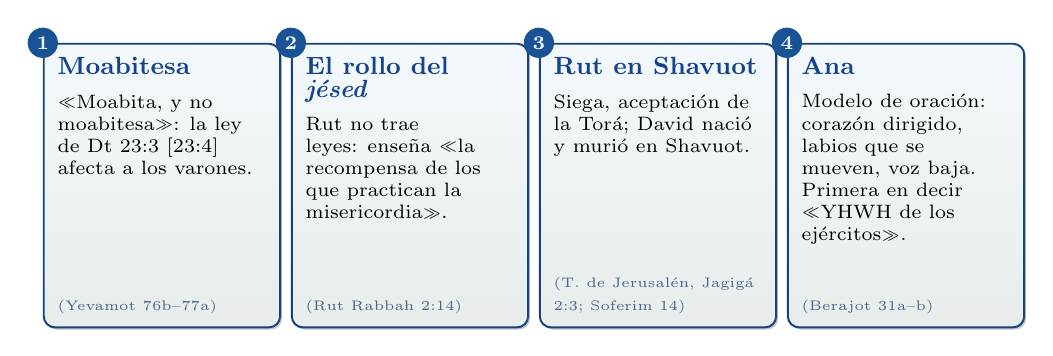
\begin{tikzpicture}
 \foreach \x/\n/\t/\d/\r in {0/1/{Moabitesa}/{«Moabita, y no moabitesa»: la ley de Dt 23:3 [23:4] afecta a los varones.}/{Yevamot 76b--77a},
   3.15/2/{El rollo del \emph{jésed}}/{Rut no trae leyes: enseña «la recompensa de los que practican la misericordia».}/{Rut Rabbah 2:14},
   6.3/3/{Rut en Shavuot}/{Siega, aceptación de la Torá; David nació y murió en Shavuot.}/{T. de Jerusalén, Jagigá 2:3; Soferim 14},
   9.45/4/{Ana}/{Modelo de oración: corazón dirigido, labios que se mueven, voz baja. Primera en decir «YHWH de los ejércitos».}/{Berajot 31a--b}}{
  \node[caja,anchor=north] (b\n) at (\x,0) {\parbox[t][3.25cm][t]{2.65cm}{\RaggedRight
    {\small\textbf{\textcolor{ladrillo}{\t}}}\\[4pt]\scriptsize \d\par\vfill{\tiny\color{sepia}(\r)}}};
  \node[circle,fill=cafe,text=piedra,font=\scriptsize\bfseries,inner sep=1.6pt] at (b\n.north west) {\n};}
\end{tikzpicture}
\end{frame}

\begin{frame}{Jueces, Saúl y David en la tradición}
\begin{columns}[t,onlytextwidth]
\begin{column}{0.49\textwidth}\scriptsize
\begin{itemize}
\item \textbf{Autoría}: «Samuel escribió su libro, Jueces y Rut»; lo completaron Gad y Natán (Bava Batra 14b--15a).
\item \textbf{Sansón}: «fue tras sus ojos; por eso le sacaron los ojos» (Mishná, Sota 1:8).
\item \textbf{Cada generación}: «Jefté en su generación es como Samuel en la suya» (Rosh Hashaná 25b).
\item \textbf{Orfa}: antepasada de Goliat (Sota 42b); \textbf{Booz} = Ibzán (Bava Batra 91a).
\end{itemize}
\end{column}
\begin{column}{0.49\textwidth}\scriptsize
\begin{itemize}
\item \textbf{Saúl y David}: «Saúl falló en una cosa, y se le contó; David en dos, y no» (Yoma 22b). Saúl se justifica (1~S 15:20); David confiesa (2~S 12:13).
\item \textbf{Profetisas}: Débora, Ana y Abigail (Meguilá 14a).
\item \textbf{Targum de Rut}: diez hambres (1:1).
\item \textbf{Josefo}, \emph{Antigüedades} 5--6: elogia el valor de Saúl en Gilboa.
\end{itemize}
\end{column}
\end{columns}
\end{frame}

\begin{frame}{En la sinagoga y en la oración}
\begin{columns}[t,onlytextwidth]
\begin{column}{0.58\textwidth}
\scriptsize\renewcommand{\arraystretch}{1.15}
\begin{tabular}{>{\RaggedRight\arraybackslash}p{2.1cm}>{\RaggedRight\arraybackslash}p{1.9cm}>{\RaggedRight\arraybackslash}p{2.9cm}}
\toprule
\textbf{Ocasión} & \textbf{Haftará} & \textbf{Conexión}\\\midrule
Beshalaj & Jue 4:4--5:31 & Débora y Éx 15\\
Nasó & Jue 13:2--25 & Sansón y el nazareo (Nm 6)\\
Jukat & Jue 11:1--33 & Jefté y Nm 21\\
Kóraj & 1~S 11:14--12:22 & Samuel y Moisés; «no desamparará»\\
Rosh Hashaná 1 & 1~S 1:1--2:10 & Ana y Sara\\
Víspera de luna nueva & 1~S 20:18--42 & Jonatán y David\\
Shavuot & Rut & Siega y Torá\\
\bottomrule
\end{tabular}
\end{column}
\begin{column}{0.39\textwidth}
\centering{\heb{אֶת־צֶמַח דָּוִד עַבְדְּךָ}}\par\smallskip
\begin{cita}[fontupper=\scriptsize\itshape]Haz brotar pronto el renuevo de David tu siervo.\fuente{(Amidá, 15.ª bendición)}\end{cita}
\scriptsize Con el lenguaje de Jer 23:5. La bendición después de comer pide por «el reino de la casa de David, tu ungido».
\end{column}
\end{columns}
\end{frame}

% ===================================================
\section{Restauración}
\begin{frame}{La promesa en esta etapa}
\centering\scriptsize\renewcommand{\arraystretch}{1.18}
\begin{tabular}{>{\RaggedRight\arraybackslash}p{1.9cm}>{\RaggedRight\arraybackslash}p{4.4cm}>{\RaggedRight\arraybackslash}p{4.6cm}}
\toprule
\textbf{Texto} & \textbf{Promesa} & \textbf{Proyección}\\\midrule
Jue 2:16, 18 & Libertadores por compasión & Is 1:26\\
Jue 7--8 & La victoria sobre Madián & Is 9:4 [9:3]; 10:26\\
Rt 4:14--17 & Un redentor y el linaje de David & Is 59:20; Ro 11:26\\
1~S 2:10 & El poder de su ungido & Sal 2:2; Lc 1:69\\
1~S 2:35 & Sacerdote fiel, casa firme & 1~S 25:28; 2~S 7:16 (Est. 4)\\
1~S 12:22 & No desamparará a su pueblo & Sal 94:14; Ro 11:1--2\\
1~S 13:14; 16:7 & Un hombre según su corazón & Jer 3:15; Hch 13:22\\
1~S 16:13 & El ungido de Belén, hijo de Isaí & Is 11:1, 10; Mi 5:2 [5:1]; Ro 15:12\\
1~S 17:46 & «Toda la tierra sabrá» & Is 55:3--5\\
\bottomrule
\end{tabular}\par\vspace{5pt}
{\small\itshape\color{sepia}YHWH «se compadecía» de su gemido (Jue 2:18): una compasión que no se apoya en el mérito.}
\end{frame}

\begin{frame}{Isaías: del día de Madián a Isaí}
\begin{columns}[t,onlytextwidth]
\begin{column}{0.49\textwidth}
\centering{\heb{וְאָשִׁיבָה שֹׁפְטַיִךְ כְּבָרִאשֹׁנָה}}\par\smallskip
\begin{cita}Restauraré tus jueces como al principio [\ldots]; entonces te llamarán Ciudad de justicia, Ciudad fiel.\fuente{(Is 1:26)}\end{cita}
\scriptsize
\begin{itemize}
\item \heb{וְאָשִׁיבָה}: raíz \emph{shuv}, la del regreso.
\item «Como en el día de Madián» (9:4 [9:3]); la peña de Oreb (10:26).
\item El niño «sobre el trono de David» (9:7 [9:6]).
\end{itemize}
\end{column}
\begin{column}{0.49\textwidth}
\centering{\heb{וְיָצָא חֹטֶר מִגֵּזַע יִשָׁי}}\par\smallskip
\begin{cita}Saldrá una vara del tronco de Isaí [\ldots] y reposará sobre él el Espíritu de YHWH.\fuente{(Is 11:1--2)}\end{cita}
\scriptsize
\begin{itemize}
\item «De Isaí», no «de David»: regreso a Belén (1~S 16).
\item Estandarte a los pueblos (11:10; Ro 15:12).
\item «Lo di por testigo a los pueblos» (55:4).
\end{itemize}
\end{column}
\end{columns}
\end{frame}

\begin{frame}{Jeremías, Oseas y Miqueas}
\begin{columns}[t,onlytextwidth]
\begin{column}{0.49\textwidth}
\begin{cita}[fontupper=\scriptsize\itshape]Levantaré a David un Renuevo justo [\ldots]. En sus días será salvo Judá, e Israel habitará confiado; y este será su nombre: YHWH, justicia nuestra.\fuente{(Jer 23:5--6)}\end{cita}
\scriptsize
\begin{itemize}
\item «Judá» = reino del sur; «Israel» = reino del norte, ya desterrado: ambos bajo el rey davídico.
\item Silo como advertencia (Jer 7:12); «pastores según mi corazón» (3:15); «David su rey» (30:9).
\end{itemize}
\end{column}
\begin{column}{0.49\textwidth}
\begin{cita}[fontupper=\scriptsize\itshape]Muchos días estarán los hijos de Israel sin rey [\ldots], sin efod y sin terafines. Después volverán y buscarán a YHWH su Dios y a David su rey.\fuente{(Os 3:4--5)}\end{cita}
\scriptsize
\begin{itemize}
\item En Oseas, «Israel» = reino del norte. Efod y terafines: Jue 8:27; 17:5. «Días de Guibeá» (Os 10:9).
\item \textbf{Mi 5:2 [5:1]}: «tú, Belén Efrata [\ldots], de ti me saldrá el que será gobernante en Israel».
\end{itemize}
\end{column}
\end{columns}
\end{frame}

\begin{frame}{Pablo, benjaminita}
\fotolado{panel_ro11.jpg}{Elaboración propia: Ro 11:1 en escritura uncial (texto NA28).}
\begin{columns}[c,onlytextwidth]
\begin{column}{0.57\textwidth}
\begin{cita}¿Ha desechado Dios a su pueblo? En ninguna manera. Porque también yo soy israelita, de la descendencia de Abraham, de la tribu de Benjamín.\fuente{(Ro 11:1)}\end{cita}
\scriptsize
\begin{itemize}
\item \grc{ἀπώσατο}: el verbo de 1~S 12:22 (LXX).
\item \textbf{Benjamín}, casi extinguido (Jue 21), tribu de Saúl y de Saulo (Hch 13:9).
\item \textbf{Hch 13:22}: «he hallado a David [\ldots], varón conforme a mi corazón».
\item \textbf{Ro 1:3}: «del linaje de David según la carne».
\item \textbf{Ro 11:26} cita Is 59:20: el \heb{גּוֹאֵל} (\emph{go'el}), título de Booz.
\end{itemize}
\end{column}
\begin{column}{0.41\textwidth}\end{column}
\end{columns}
\end{frame}

% ===================================================
\AtBeginSection[]{}
\section{Síntesis}
\begin{frame}{Síntesis}
\begin{tcolorbox}[colback=piedra,colframe=ladrillo,boxrule=1pt,arc=3pt,fontupper=\small]
\textbf{\textcolor{cafe}{De los Jueces a David:}} el pueblo llamado a ser reino de sacerdotes quiso ser «como todas las naciones» y se corrompió desde dentro, hasta convertirse en Sodoma en Guibeá. Dios, con todo, se compadeció, guardó un remanente (Débora, Rut, Ana, Samuel, Jonatán, David) y anunció un rey ungido salido de Belén. Sobre esa promesa descansa la esperanza de Isaías en el renuevo de Isaí, la de Jeremías en el Renuevo justo y la de Oseas en «David su rey», y de ella toma Pablo su respuesta: «No ha desechado Dios a su pueblo» (Ro 11:2).
\end{tcolorbox}
\scriptsize\renewcommand{\arraystretch}{1.2}
\begin{tabular}{>{\RaggedRight\arraybackslash}p{3.0cm}>{\RaggedRight\arraybackslash}p{8.3cm}}
\toprule
\textbf{Eje} & \textbf{Lo que deja esta etapa}\\\midrule
Vocación quebrada & Jue 17--21; 1~S 2:12--17; 8:5, 20\\
Remanente & Jue 5; Rt 1:16; 1~S 1--2; 7; 12:23; 17:46\\
Restauración & Jue 2:18; Rt 4:14--17; 1~S 2:10, 35; 12:22; 16:13\\
Proyección & Is 1:26; 11:1; Jer 23:5--6; Os 3:4--5; Mi 5:2 [5:1]; Ro 11:1--5\\
\bottomrule
\end{tabular}
\end{frame}

\begin{frame}{Hacia el Estudio 4}
\begin{columns}[c,onlytextwidth]
\begin{column}{0.55\textwidth}
\begin{cita}Y vinieron los hombres de Judá y ungieron allí a David por rey sobre la casa de Judá.\fuente{(2~S 2:4)}\end{cita}
\small Un rey ungido, pero un reino incompleto: David reina en Hebrón sobre Judá, y la casa de Saúl conserva el resto de Israel. Quedan por venir \destacar{Jerusalén}, \destacar{el arca} y \destacar{la casa eterna}.
\end{column}
\begin{column}{0.42\textwidth}
\begin{tcolorbox}[colback=cafe,colframe=cafeosc,coltext=piedra,boxrule=0.8pt,arc=3pt,fontupper=\small]
\textbf{Estudio 4}\par\smallskip
De David a la división del reino: Jerusalén, pacto davídico (2~S 7), Salomón y el Primer Templo, y la división entre Israel (norte) y Judá (sur).
\end{tcolorbox}
\end{column}
\end{columns}
\end{frame}

\begin{frame}{Para la reflexión}
\small
\begin{enumerate}
\item El estribillo «cada uno hacía lo que bien le parecía» (Jue 21:25) retoma Dt 12:8. ¿Qué supone hoy vivir conforme a «lo recto ante los ojos de YHWH»?
\item Israel pidió un rey «como todas las naciones» (1~S 8:5). ¿Bajo qué formas aparece hoy el deseo de asemejarse al entorno?
\item Rut dijo «tu pueblo será mi pueblo, y tu Dios mi Dios». ¿Qué enseña su orden a los creyentes de las naciones (Ro 11:17--18)?
\item «Obedecer es mejor que el sacrificio» (1~S 15:22). ¿Cómo distinguir el culto como obediencia del culto como medio?
\item ¿Qué relación hay entre la preservación de Benjamín (Jue 21) y el remanente de Ro 11:1--5?
\end{enumerate}
\end{frame}

% ===================================================
\section{Glosario}
\begin{frame}{Glosario}
\begin{columns}[t,onlytextwidth]
\begin{column}{0.49\textwidth}\scriptsize
\textbf{Eben-ezer} (\heb{אֶבֶן הָעָזֶר}): «piedra de la ayuda» (1~S 7:12).\par\smallskip
\textbf{Go'el} (\heb{גֹּאֵל}): pariente redentor (Rt 4:14; Is 59:20).\par\smallskip
\textbf{Icabod} (\heb{אִי־כָבוֹד}): «¿dónde está la gloria?» (1~S 4:21).\par\smallskip
\textbf{Jésed} (\heb{חֶסֶד}): lealtad amorosa (Rt 1:8; 3:10).\par\smallskip
\textbf{Kejol ha-goyim} (\heb{כְּכָל־הַגּוֹיִם}): «como todas las naciones» (1~S 8:5).\par\smallskip
\textbf{Mashíaj} (\heb{מָשִׁיחַ}; \grc{χριστός}): ungido (1~S 2:10).
\end{column}
\begin{column}{0.49\textwidth}\scriptsize
\textbf{Naguid} (\heb{נָגִיד}): príncipe, designado (1~S 10:1).\par\smallskip
\textbf{Nazir} (\heb{נָזִיר}): consagrado por voto (Nm 6; Jue 13:5).\par\smallskip
\textbf{Seraním} (\heb{סְרָנִים}): príncipes filisteos (Jue 3:3).\par\smallskip
\textbf{Shofet} (\heb{שֹׁפֵט}): juez, libertador (Jue 2:16).\par\smallskip
\textbf{Tsémaj} (\heb{צֶמַח}): renuevo davídico (Jer 23:5).\par\smallskip
\textbf{Yashar be-einav} (\heb{הַיָּשָׁר בְּעֵינָיו}): «lo recto ante sus ojos» (Jue 21:25).
\end{column}
\end{columns}
\end{frame}

% ===================================================
\section{Referencias}
\begin{frame}[allowframebreaks]{Referencias}
\tiny
\refapa{\emph{Biblia Hebraica Stuttgartensia} (5.ª ed.). (1997). Deutsche Bibelgesellschaft.}
\refapa{Block, D.~I. (1999). \emph{Judges, Ruth} (New American Commentary, Vol. 6). Broadman \& Holman.}
\refapa{Bunimovitz, S., \& Lederman, Z. (2009). The archaeology of border communities: Renewed excavations at Tel Beth-Shemesh, Part 1: The Iron Age. \emph{Near Eastern Archaeology, 72}(3), 114--142.}
\refapa{Cohen, A. (Ed.). (1965). \emph{The minor tractates of the Talmud}. Soncino Press.}
\refapa{Cross, F.~M., \& Freedman, D.~N. (1997). \emph{Studies in ancient Yahwistic poetry} (2.ª ed.). Eerdmans.}
\refapa{Cross, F.~M., Parry, D.~W., Saley, R.~J., \& Ulrich, E. (2005). \emph{Qumran Cave 4.XII: 1--2 Samuel} (Discoveries in the Judaean Desert 17). Clarendon Press.}
\refapa{Danby, H. (Trad.). (1933). \emph{The Mishnah}. Oxford University Press.}
\refapa{Dothan, T. (1982). \emph{The Philistines and their material culture}. Yale University Press.}
\refapa{Epstein, I. (Ed.). (1935--1948). \emph{The Babylonian Talmud}. Soncino Press.}
\refapa{Faust, A. (2006). \emph{Israel's ethnogenesis: Settlement, interaction, expansion and resistance}. Equinox.}
\refapa{Feldman, M., Master, D.~M., Bianco, R.~A., Burri, M., Stockhammer, P.~W., Mittnik, A., Aja, A.~J., Jeong, C., \& Krause, J. (2019). Ancient DNA sheds light on the genetic origins of early Iron Age Philistines. \emph{Science Advances, 5}(7), eaax0061.}
\refapa{Finkelstein, I. (1988). \emph{The archaeology of the Israelite settlement}. Israel Exploration Society.}
\refapa{Finkelstein, I., Bunimovitz, S., \& Lederman, Z. (1993). \emph{Shiloh: The archaeology of a biblical site}. Institute of Archaeology, Tel Aviv University.}
\refapa{Finkelstein, I., \& Fantalkin, A. (2012). Khirbet Qeiyafa: An unsensational archaeological and historical interpretation. \emph{Tel Aviv, 39}(1), 38--63.}
\refapa{Freedman, H., \& Simon, M. (Eds.). (1939). \emph{Midrash Rabbah}. Soncino Press.}
\refapa{Garfinkel, Y., Kreimerman, I., \& Zilberg, P. (2016). \emph{Debating Khirbet Qeiyafa: A fortified city in Judah from the time of King David}. Israel Exploration Society.}
\refapa{Gitin, S., Dothan, T., \& Naveh, J. (1997). A royal dedicatory inscription from Ekron. \emph{Israel Exploration Journal, 47}(1--2), 1--16.}
\refapa{Guggenheimer, H.~W. (1998). \emph{Seder Olam: The rabbinic view of biblical chronology}. Jason Aronson.}
\refapa{Harrington, D.~J., \& Saldarini, A.~J. (1987). \emph{Targum Jonathan of the Former Prophets} (The Aramaic Bible, Vol. 10). Michael Glazier.}
\refapa{Hesse, B., \& Wapnish, P. (1997). Can pig remains be used for ethnic diagnosis in the ancient Near East? En N.~A. Silberman \& D.~B. Small (Eds.), \emph{The archaeology of Israel}. Sheffield Academic Press.}
\refapa{Josefo, F. (1987). \emph{The works of Josephus} (W. Whiston, Trad.). Hendrickson.}
\refapa{Levine, É. (1973). \emph{The Aramaic version of Ruth}. Biblical Institute Press.}
\refapa{Maeir, A.~M., Wimmer, S.~J., Zukerman, A., \& Demsky, A. (2008). A late Iron Age I/early Iron Age IIA Old Canaanite inscription from Tell eṣ-Ṣâfī/Gath, Israel. \emph{Bulletin of the American Schools of Oriental Research, 351}, 39--71.}
\refapa{Mazar, A. (1990). \emph{Archaeology of the land of the Bible, 10,000--586 B.C.E.} Doubleday.}
\refapa{McCarter, P.~K. (1980). \emph{I Samuel} (Anchor Bible, Vol. 8). Doubleday.}
\refapa{Moo, D.~J. (1996). \emph{The epistle to the Romans}. Eerdmans.}
\refapa{Neusner, J. (Trad.). (1982--1994). \emph{The Talmud of the Land of Israel}. University of Chicago Press.}
\refapa{\emph{Novum Testamentum Graece} (28.ª ed.). (2012). Deutsche Bibelgesellschaft.}
\refapa{ONE FOR ISRAEL Ministry. (2025, 3 de julio). \emph{What does «all Israel will be saved» mean in Romans 11?} \url{https://www.oneforisrael.org/what-does-all-israel-will-be-saved-mean-in-romans-11/}}
\refapa{Rahlfs, A., \& Hanhart, R. (Eds.). (2006). \emph{Septuaginta} (ed. rev.). Deutsche Bibelgesellschaft.}
\refapa{Sacks, J. (Trad.). (2009). \emph{The Koren Siddur}. Koren Publishers.}
\refapa{Stager, L.~E. (1985). The archaeology of the family in ancient Israel. \emph{Bulletin of the American Schools of Oriental Research, 260}, 1--35.}
\end{frame}
\end{document}
